\begin{frame}
\frametitle{Labs proposed on another platform}
  \begin{columns}
    \column{0.7\textwidth}
    In addition to the BeagleBone and the STM32MP157D-DK1 you can also run
    most labs on the Beagleplay board.\\
    \vspace{1em}
    Lab instructions are available at\\
    {\small \url{https://bootlin.com/doc/training/embedded-linux-beagleplay/}}
    \column{0.3\textwidth}
    \begin{center}
      
\includegraphics[width=\textwidth]{../slides/beagleplay-board/beagle_logo_326x60.png}\\
      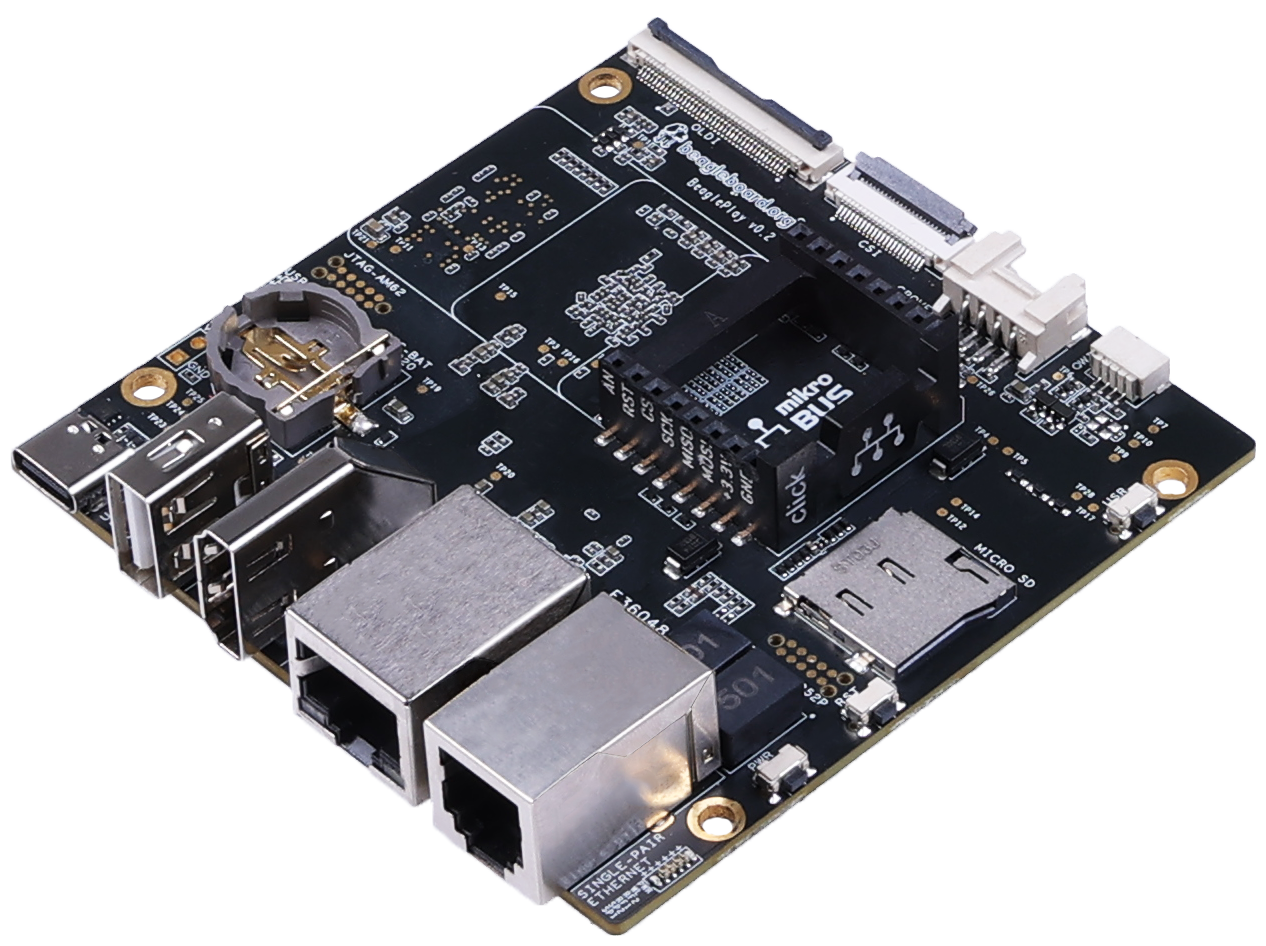
\includegraphics[width=\textwidth]{../slides/beagleplay-board/beagleplay.png}\\
      \includegraphics[width=0.5\textwidth]{common/open-source-hardware-logo.pdf}
    \end{center}
  \end{columns}
\end{frame}
